% !TeX spellcheck = en_US
% !TeX encoding = UTF-8
\documentclass{beamer}

\mode<presentation> { \usetheme{Madrid} }

\usepackage{graphicx, graphics}
\usepackage[notocbib]{apacite}
\usepackage[style=iso]{datetime2}
\usepackage{enumerate}
\providecommand\thispdfpagelabel[1]{}
\DeclareGraphicsExtensions{.pdf, .png, .jpg, .gif}

\AtBeginSection[]
{
    \begin{frame}
        \vfill
        \centering
        \begin{beamercolorbox}[sep=8pt,center,shadow=true,rounded=true]{title}
            \usebeamerfont{title}
            \thesection. \insertsectionhead
            \par
        \end{beamercolorbox}
        \vfill
    \end{frame}
}

\AtBeginSubsection[]
{
    \begin{frame}
        \vfill
        \centering
        \begin{beamercolorbox}[sep=8pt, center, shadow=true, rounded=true]{title}
            \usebeamerfont{title}
            \thesection. \insertsectionhead
            \par
        \end{beamercolorbox}
        \begin{beamercolorbox}[sep=6pt, center, shadow=true, rounded=true]{title}
            \usebeamerfont{subtitle}
            \thesection.\thesubsection. \insertsubsectionhead
            \par
        \end{beamercolorbox}
        \vfill
    \end{frame}
}

\AtBeginSubsubsection[]
{
    \begin{frame}
        \vfill
        \centering
        \begin{beamercolorbox}[sep=8pt, center, shadow=true, rounded=true]{title}
            \usebeamerfont{title}
            \thesection. \insertsectionhead
            \par
        \end{beamercolorbox}
        \begin{beamercolorbox}[sep=6pt, center, shadow=true, rounded=true]{title}
            \usebeamerfont{subtitle}
            \thesection.\thesubsection. \insertsubsectionhead
            \par
        \end{beamercolorbox}
        \begin{beamercolorbox}[sep=4pt, center, shadow=true, rounded=true]{title}
            \usebeamerfont{subsubtitle}
            \thesection.\thesubsection.\thesubsubsection. \insertsubsubsectionhead
            \par
        \end{beamercolorbox}
        \vfill
    \end{frame}
}

\title[PTB]{Metagenome Analysis of Preterm Birth}

\author[Jaewoong Lee]
{
    Jaewoong Lee
    \and
    Semin Lee
}

\institute[UNIST BME]
{
    Department of Biomedical Engineering
    \newline
    Ulsan National Institute of Science and Technology
    \medskip
    \newline
    \textit{jwlee230@unist.ac.kr}
}

\date{\today}

\begin{document}
    \begin{frame}
        \titlepage
    \end{frame}

	\begin{frame}
        \frametitle{Overview}
        \tableofcontents[hideallsubsections]
    \end{frame}

    \section{Introduction}
    \begin{frame}
        \frametitle{Microbiome}

        \begin{itemize}
            \item Microbiota: the microorganisms which live inside \& on humans \cite{micro1}
            \item Microbiome: $10^{13}$ to $10^{14}$ microorganisms whose which collective genome \cite{micro2}
        \end{itemize}

        \begin{figure}
            \includegraphics[width=0.3 \linewidth]{figures/microbiome.jpg}
            \caption{Concept of a core human microbiome \protect \cite{micro1}}
        \end{figure}
    \end{frame}

    \begin{frame}
        \frametitle{rRNA}

        \begin{itemize}
            \item Ribosomal RNA
            \item Well-known as a key to phylogeny \cite{rrna1}
        \end{itemize}
    \end{frame}

    \begin{frame}
        \frametitle{Preterm Birth (PTB)}

        PTB:
        \begin{enumerate}
            \item PTB $<$ 37 GW (Gestational week)
            \item Normal $\ge$ 37 GW
        \end{enumerate}

        Detailed PTB:
        \begin{enumerate}
            \item Early PTB $<$ 34 GW
            \item 34 GW $\le$ Late PTB $<$ 37 GW
            \item Normal $\ge$ 37 GW
        \end{enumerate}

        \cite{premature1, premature2}
    \end{frame}

    \section{Materials}
    \begin{frame}
        \frametitle{16S rRNA Sequencing}

        \textbf{16S rRNA sequencing} is the \textit{reference method} for bacterial taxonomy \& identification \cite{16S1}

        Three main reasons \cite{16S2}:
        \begin{itemize}
            \item 16S rRNA exists in almost all bacteria
            \item Functions of the 16S rRNA has not changed over evolution.
            \item 16S rRNA is large enough for bioinformatics
        \end{itemize}
    \end{frame}

    \begin{frame}
        \frametitle{Data Composition}
        \begin{itemize}
            \item JBNU/Helixco data
            \begin{itemize}
                \item First data
                \item Second data
                \item Stool data
            \end{itemize}
        \end{itemize}

        \begin{table}
            \centering
            \caption{Sample Information}
            \begin{tabular}{c|ccc}
    Data & Participants & Samples & Remarks \\ \hline
    First & 24 & 107 & - \\
    Second & 35 & 288 & - \\
    Stool & 63 & 126 & Stool \\
    EBI & 18 & 1016 & Only Normal \\
    HMP & 1572 & 9205 & Only Premature \\
\end{tabular}

        \end{table}
    \end{frame}

    \section{Methods}
    \begin{frame}
        \frametitle{Qiime 2 Workflow}

        \begin{figure}
            \includegraphics[width=0.8 \linewidth]{figures/qiime.png}
            \caption{QIIME 2 workflow \protect\cite{qiime1, qiime2, qiime3}}
        \end{figure}
    \end{frame}

    \section{Results}
    \subsection{Taxonomy Overview}
    \begin{frame}
        \frametitle{Proportion Distribution}

        \begin{columns}
            \begin{column}{0.4 \linewidth}
                \begin{block}{Proportion}
                    \begin{itemize}
                        \item Minimum: 0.0
                        \item Mean: 0.00008
                        \item Median: 0.0
                        \item Maximum: 0.793
                    \end{itemize}
                \end{block}
            \end{column}

            \begin{column}{0.4 \linewidth}
                \begin{block}{Proportion without Zero}
                    \begin{itemize}
                        \item Minimum: 0.00002
                        \item Mean: 0.00008
                        \item Median: 0.00153
                        \item Maximum: 0.793
                    \end{itemize}
                \end{block}
            \end{column}
        \end{columns}

        \begin{figure}
            \includegraphics[width=0.5 \linewidth]{figures/Step53_Proportion/everything.DADA2.homd.uncorrected.pdf}
            \caption{Proportion distribution}
        \end{figure}
    \end{frame}

    \begin{frame}
        \frametitle{Microbial community with Proportion}

        \begin{figure}
            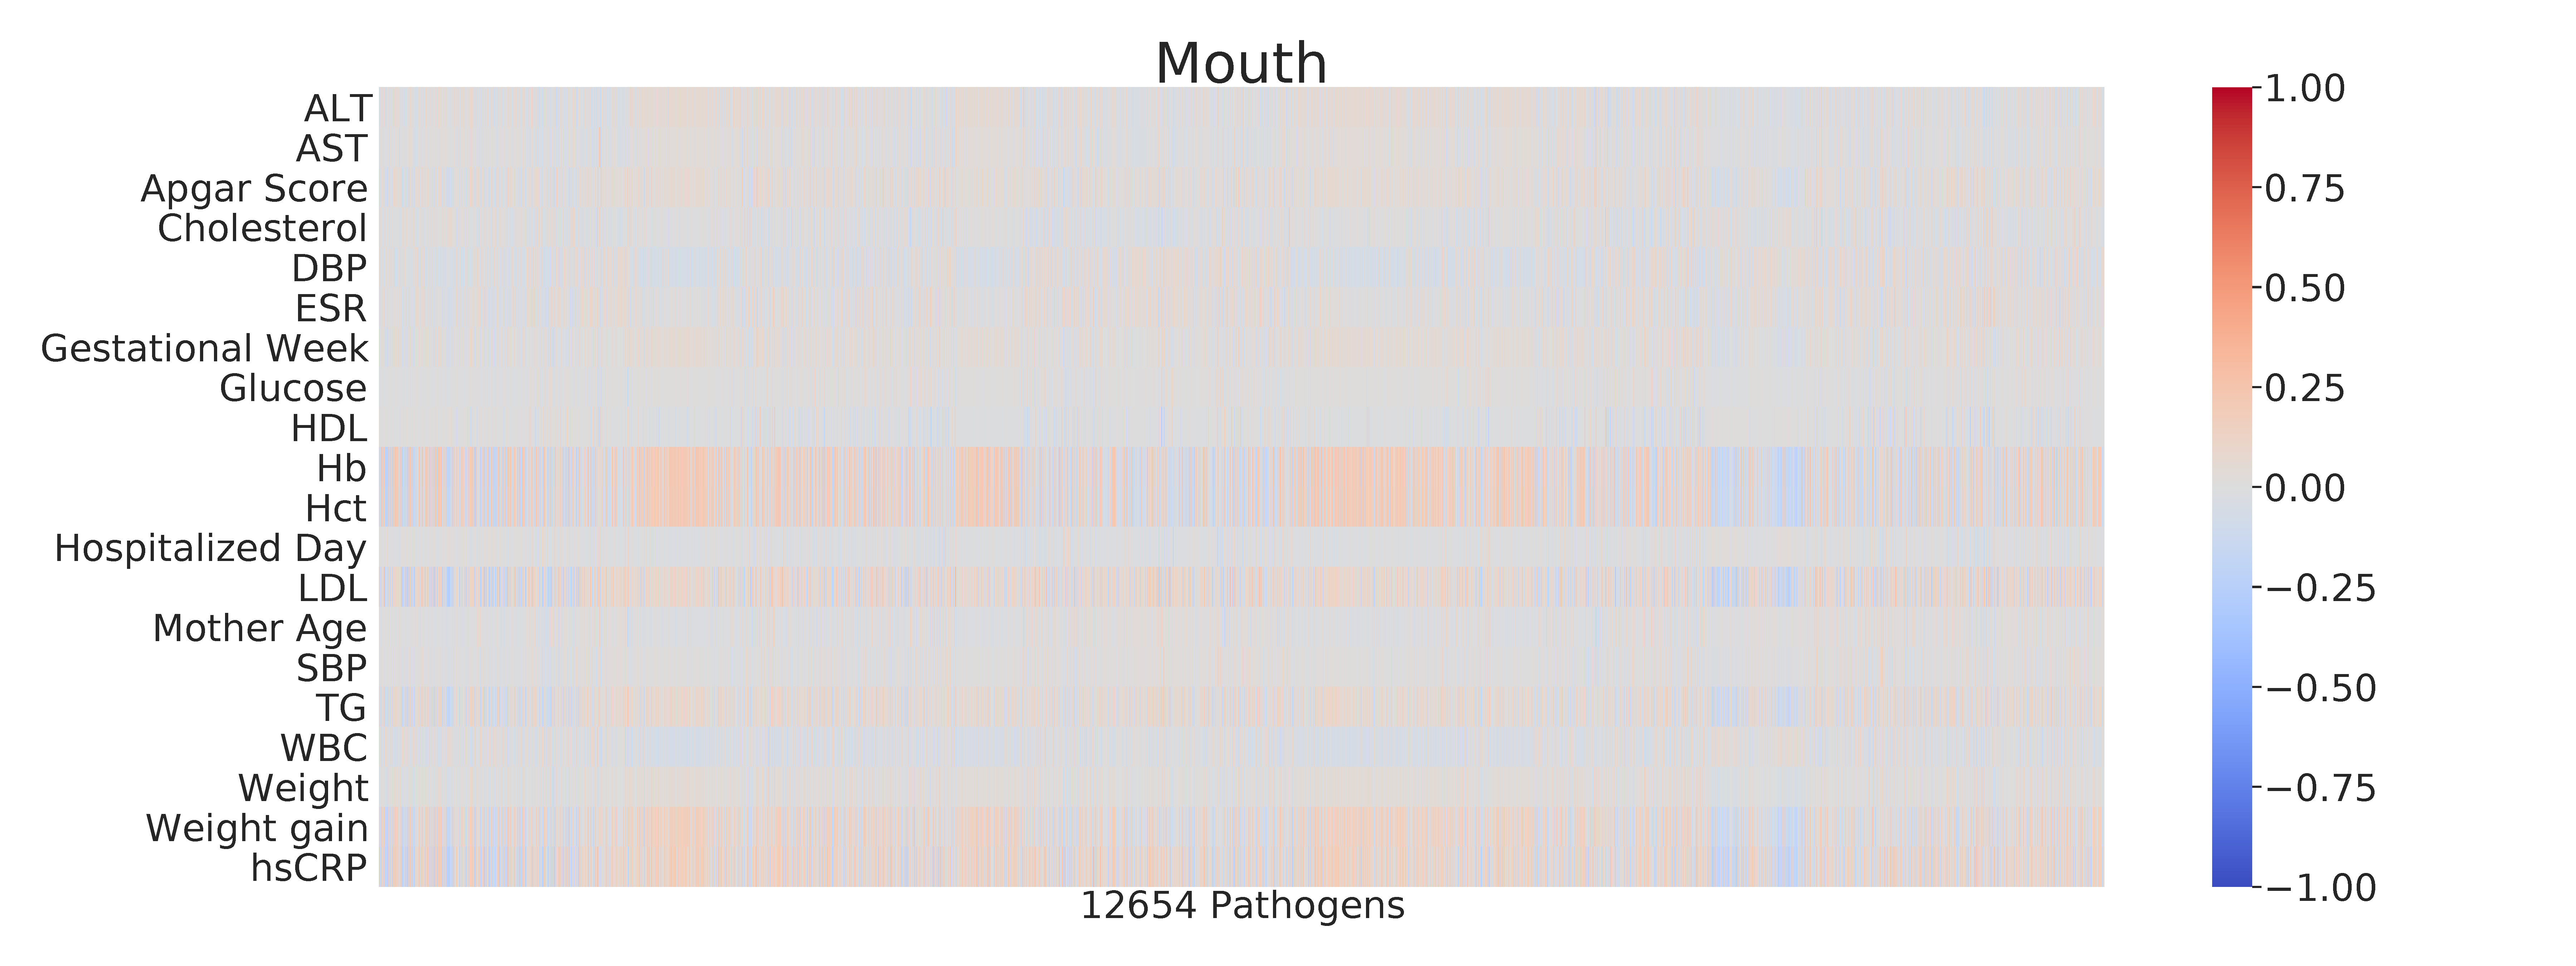
\includegraphics[width=0.6 \linewidth]{figures/Step60_Proportion/everything.DADA2.homd.uncorrected/Mouth.pdf}
            \caption{Microbial community with Proportion}
        \end{figure}
    \end{frame}

    \begin{frame}
        \frametitle{t-SNE with Proportion}

        \begin{figure}
            $\begin{array}{cc}
                \includegraphics[width=0.4 \linewidth]{figures/tSNE_Proportion/everything.DADA2.homd.uncorrected/All+Detail_Premature.pdf}
                &
                \includegraphics[width=0.4 \linewidth]{figures/tSNE_Proportion/everything.DADA2.homd.uncorrected/Mouth+Detail_Premature.pdf}
                \\
                \mbox{(a) All} & \mbox{(b) Mother Mouth} \\
            \end{array}$
            \caption{t-SNE plot of Proportion with PTB}
        \end{figure}
    \end{frame}

    \begin{frame}[allowframebreaks]
        \frametitle{Notable Taxa}

        \begin{block}{\textit{Streptococcus} spp.}
            \begin{itemize}
                \item \textit{S. mutans}: pathogen of dental caries
                \item Membrane vesicles of Group B \textit{Streptococcus} disrupt feto-maternal barrier \cite{streptococcus-1}. \\
                    $\therefore$ Leading to PTB
            \end{itemize}
        \end{block}

        \begin{block}{\textit{Neisseria} spp.}
            \begin{itemize}
                \item \textit{N.} colonize the mucosal surfaces of many animals.
                \item Only two pathogens in 11 known species
                    \begin{itemize}
                        \item \textit{N. meningitidis}: Meningitis \& Sepsis
                        \item \textit{N. gonorrhoeae}: Gonorrhea (sexual transmitted disease)
                    \end{itemize}
                \item \textit{N. gonorrhoeae} results adverse pregnancy outcomes \cite{neisseria-1}.
            \end{itemize}
        \end{block}

        \begin{block}{\textit{Haemophilus} spp.}
            \begin{itemize}
                \item \textit{H.} inhabit the mucous membranes \\
                    of upper respiratory tract, mouth, vagina, \& intestinal tract.
                \item \textit{H. influenzae}: Influenza
                \item PTB caused by \textit{H. influenzae} \cite{haemophilus-1} and \textit{H. parainfluenzae} \cite{haemophilus-2}.
            \end{itemize}
        \end{block}

        \begin{block}{\textit{R. mucilaginosa}}
            \begin{itemize}
                \item \textit{Rhodotorula mucilaginosa}
                \item \textit{R.} is a genus of pigmented yeasts.
                \item Catheter-related bloodstream infection due to \textit{R. mucilaginosa} \cite{rhodotorula-1}.
                \item $\therefore$ \textit{Rhodotorula} bloodstream infections
            \end{itemize}
        \end{block}

        \begin{block}{\textit{Gemella} spp.}
            \begin{itemize}
                \item \textit{G.} bacteria are primarily found in mucous membranes of human \\
                    \textit{e.g.} oral cavity \& upper digestive tract.
                \item \textit{G. haemolysans} causes endocarditis \cite{gemella-2}.
                \item Women who have PTB also have significant lower level of \textit{G.} \cite{gemella-1}.
            \end{itemize}
        \end{block}
    \end{frame}

    \subsection{Diversity Index}
    \begin{frame}
        \frametitle{Diversity Index}

        \begin{figure}
            \includegraphics[width=0.6 \linewidth]{figures/phylogenic.jpg}
            \caption{Three dimensions of phylogenetic information \protect\cite{phylogenetic1}}
        \end{figure}

        \begin{itemize}
            \item A quantitative measure that shows richness, divergence, and regularity \cite{phylogenetic1}
            \item Alpha diversity: the richness of taxa \textbf{at a single community}
            \item Beta diversity: taxonomy differentiation \textbf{between communities}
        \end{itemize}
    \end{frame}

    \subsubsection{Alpha-diversity}
    \begin{frame}[allowframebreaks]
        \frametitle{Violin Plot with Alpha-diversity}

        \begin{figure}
            $\begin{array}{cc}
                \includegraphics[width=0.4 \linewidth]{figures/AlphaDiversity/everything.DADA2/All+Detail_Premature+faith_pd.pdf}
                &
                \includegraphics[width=0.4 \linewidth]{figures/AlphaDiversity/everything.DADA2/Mouth+Detail_Premature+faith_pd.pdf}
                \\
                \mbox{(a) All} & \mbox{(b) Mother Mouth} \\
            \end{array}$
            \caption{Detail premature \& Faith's PD}
        \end{figure}

        \begin{figure}
            $\begin{array}{cc}
                \includegraphics[width=0.4 \linewidth]{figures/AlphaDiversity/everything.DADA2/All+Detail_Premature+observed_otus.pdf}
                &
                \includegraphics[width=0.4 \linewidth]{figures/AlphaDiversity/everything.DADA2/Mouth+Detail_Premature+observed_otus.pdf}
                \\
                \mbox{(a) All} & \mbox{(b) Mother Mouth} \\
            \end{array}$
            \caption{Detail premature \& Observed OTUs}
        \end{figure}

        \begin{figure}
            $\begin{array}{cc}
                \includegraphics[width=0.4 \linewidth]{figures/AlphaDiversity/everything.DADA2/All+Detail_Premature+pielou_e.pdf}
                &
                \includegraphics[width=0.4 \linewidth]{figures/AlphaDiversity/everything.DADA2/Mouth+Detail_Premature+pielou_e.pdf}
                \\
                \mbox{(a) All} & \mbox{(b) Mother Mouth} \\
            \end{array}$
            \caption{Detail premature \& Pielou Evenness}
        \end{figure}

        \begin{figure}
            $\begin{array}{ccc}
                \includegraphics[width=0.4 \linewidth]{figures/AlphaDiversity/everything.DADA2/Mouth+Detail_Premature+shannon.pdf}
                &
                \includegraphics[width=0.4 \linewidth]{figures/AlphaDiversity/everything.DADA2/Neonate-3day+Detail_Premature+shannon.pdf}
                \\
                \mbox{(a) All} & \mbox{(b) Mother Mouth} \\
            \end{array}$
            \caption{Detail premature \& Shannon Entropy}
        \end{figure}
    \end{frame}

    \subsubsection{Beta-diversity}
    \begin{frame}[allowframebreaks]
        \frametitle{Beta-diversity t-SNE plots}

        \begin{figure}
            $\begin{array}{cc}
                \includegraphics[width=0.4 \linewidth]{figures/BetaDiversity/everything.DADA2.homd.uncorrected/Mouth+Detail_Premature+braycurtis.pdf}
                &
                \includegraphics[width=0.4 \linewidth]{figures/BetaDiversity/everything.DADA2.homd.uncorrected/Mouth+Detail_Premature+euclidean.pdf}
                \\
                \mbox{(a) Bray-Curtis} & \mbox{(b) Euclidean} \\
            \end{array}$
            \caption{Beta-diversity t-SNE plots}
        \end{figure}
    \end{frame}

    \subsection{Taxonomy Analyses}
    \subsubsection{Differentially Abundant Taxa}
    \begin{frame}[allowframebreaks]
        \frametitle{Volcano plots}

        \begin{figure}
            $\begin{array}{cc}
                \includegraphics[width=0.4 \linewidth]{figures/Step63/everything.DADA2.homd.Mouth.pdf}
                &
                \includegraphics[width=0.4 \linewidth]{figures/Step63/everything.DADA2.homd.Mouth.PTB.pdf}
                \\
                \mbox{(a) Early PTB vs. other} & \mbox{(b) PTB vs. Normal} \\
            \end{array}$
            \caption{DAT in Mouth}
        \end{figure}

        \begin{figure}
            $\begin{array}{ccc}
                \includegraphics[width=0.3 \linewidth]{figures/Step63/everything.DADA2.homd.Mouth.EL.pdf}
                &
                \includegraphics[width=0.3 \linewidth]{figures/Step63/everything.DADA2.homd.Mouth.EF.pdf}
                &
                \includegraphics[width=0.3 \linewidth]{figures/Step63/everything.DADA2.homd.Mouth.LF.pdf}
                \\
                \mbox{(a) Early vs. Late} & \mbox{(b) Early vs. Normal} & \mbox{(c) Late vs. Normal} \\
            \end{array}$
            \caption{DAT in Mouth}
        \end{figure}
    \end{frame}

    \begin{frame}
        \frametitle{Venn Diagrams}

        \begin{figure}
            \includegraphics[width=\linewidth]{figures/Step68_Updown/everything.DADA2.homd.Mouth.pdf}
            \caption{DAT Upset plot}
        \end{figure}

        \begin{block}{Union of DAT}
            A total of 20 taxa selected as DAT.
        \end{block}
    \end{frame}

    \begin{frame}[allowframebreaks]
        \frametitle{Violin Plots}

        \begin{columns}
            \begin{column}{0.4 \linewidth}
                \begin{figure}
                    \includegraphics[width=\linewidth]{figures/Step71_Proportion/everything.DADA2.homd.Mouth/C. durum.pdf}
                    \caption{\textit{C. durum}}
                \end{figure}
            \end{column}
            \begin{column}{0.6 \linewidth}
                \begin{block}{\textit{C. durum}}
                    \begin{itemize}
                        \item \textit{Corynebacterium durum}
                        \item Poly-microbial interactions \\
                            $\Rightarrow$ Oral mucosal \& Gingival cells \cite{Corynebacterium-1}.
                        \item Synergism between \textit{C.} \& \textit{Streptococcus} in oral commensals \cite{Corynebacterium-2}.
                    \end{itemize}
                \end{block}
            \end{column}
        \end{columns}

        \begin{columns}
            \begin{column}{0.4 \linewidth}
                \begin{figure}
                    \includegraphics[width=\linewidth]{figures/Step71_Proportion/everything.DADA2.homd.Mouth/P. gingivalis.pdf}
                    \caption{\textit{P. gingivalis}}
                \end{figure}
            \end{column}
            \begin{column}{0.6 \linewidth}
                \begin{block}{\textit{P. gingivalis}}
                    \begin{itemize}
                        \item \textit{Porphyromonas gingivalis}
                        \item \textit{P. gingivalis} is well-known periodontitis pathogen.
                        \item \textit{P. gingivalis} is associated with bacterial vaginosis \cite{Porphyromonas-1}.
                        \item \textit{P. gingivalis} $\Rightarrow$ Adverse prenancy outcomes \cite{Porphyromonas-2}.
                    \end{itemize}
                \end{block}
            \end{column}
        \end{columns}

        \begin{block}{\textit{Prevotella} spp.}
            \begin{itemize}
                \item \textit{P.} interactions with human health \cite{Prevotella-1}.
                \item \textit{P.} spp. might have different role in PTB \cite{Prevotella-2}.
                \item \textit{P.} spp. are associated with human infections \cite{Prevotella-4}.
            \end{itemize}
        \end{block}
        \pagebreak

        \begin{columns}
            \begin{column}{0.4 \linewidth}
                \begin{figure}
                    \includegraphics[width=\linewidth]{figures/Step71_Proportion/everything.DADA2.homd.Mouth/P. dentalis.pdf}
                    \caption{\textit{P. dentalis}}
                \end{figure}
            \end{column}
            \begin{column}{0.6 \linewidth}
                \begin{block}{\textit{P. dentalis}}
                    \begin{itemize}
                        \item \textit{Prevotella dentalis}
                        \item \textit{P. dentalis} is observed as colorectal cancer-promoting bacterium \cite{Prevotella-3}.
                    \end{itemize}
                \end{block}
            \end{column}
        \end{columns}

        \begin{columns}
            \begin{column}{0.4 \linewidth}
                \begin{figure}
                    \includegraphics[width=\linewidth]{figures/Step71_Proportion/everything.DADA2.homd.Mouth/P. pleuritidis.pdf}
                    \caption{\textit{P. pleuritidis}}
                \end{figure}
            \end{column}
            \begin{column}{0.6 \linewidth}
                \begin{block}{\textit{P. pleuritidis}}
                    \begin{itemize}
                        \item \textit{Prevotella pleuritidis}
                        \item \textit{P. pleuritidis} causes lung abscess \cite{Prevotella-5}.
                        \item \textit{P. pleuritidis} is abundant in oral microbiome of smokers \cite{Prevotella-6}.
                        \item \textit{P. pleuritidis} associated with gastric cancer \cite{Prevotella-7}.
                    \end{itemize}
                \end{block}
            \end{column}
        \end{columns}
    \end{frame}

    \subsection{Machine Learning}
    \begin{frame}
        \frametitle{ML algorithm comparison}

        \begin{figure}
            \includegraphics[width=\linewidth]{figures/ML.png}
            \caption{Classification Comparison \protect\cite{sklearn1}}
        \end{figure}
    \end{frame}

    \begin{frame}
        \frametitle{Oversampling}

        \begin{block}{SMOTE \cite{SMOTE1}}
            \begin{itemize}
                \item Synthetic Minority Oversampling Technique
                \item An algorithm that makes pseudo-sample
                \item Using $K$-Nearest Neighbor algorithm
            \end{itemize}
        \end{block}

        \begin{figure}
            \includegraphics[width=0.8 \linewidth]{figures/SMOTE.png}
            \caption{Workflow of SMOTE}
        \end{figure}
    \end{frame}

    \subsubsection{Random Forest Classifier on Proportion}
    \begin{frame}[allowframebreaks]
        \frametitle{Random Forest with (Early vs. Late vs. Normal)}

        \begin{figure}
            \includegraphics[width=0.8 \linewidth]{figures/RandomForest_Proportion/RF.DADA2.homd.Mouth/metrics.pdf}
            \caption{RF evaluations with feature counts}
        \end{figure}

        \begin{figure}
            \includegraphics[width=0.5 \linewidth]{figures/RandomForest_Proportion/RF.DADA2.homd.Mouth/heatmap.pdf}
            \caption{RF confusion matrix}
        \end{figure}

        \begin{figure}
            \includegraphics[width=0.8 \linewidth]{figures/RandomForest_Proportion/RF.DADA2.homd.Mouth/importances.pdf}
            \caption{RF importances}
        \end{figure}

        \begin{block}{Highest Importances}
            \begin{enumerate}
                \item \textit{L. umeaense}
                \item \textit{S. sp. HMT 442}
                \item \textit{V. dispar}
            \end{enumerate}
        \end{block}
    \end{frame}

    \begin{frame}[allowframebreaks]
        \frametitle{Random Forest with (Early vs. Late + Normal)}

        \begin{figure}
            \includegraphics[width=0.8 \linewidth]{figures/RandomForest_Proportion/RF-two.DADA2.homd.Mouth/metrics.pdf}
            \caption{RF evaluations with feature counts}
        \end{figure}

        \begin{figure}
            \includegraphics[width=0.5 \linewidth]{figures/RandomForest_Proportion/RF-two.DADA2.homd.Mouth/heatmap.pdf}
            \caption{RF confusion matrix}
        \end{figure}

        \begin{figure}
            \includegraphics[width=0.8 \linewidth]{figures/RandomForest_Proportion/RF-two.DADA2.homd.Mouth/importances.pdf}
            \caption{RF importances}
        \end{figure}

        \begin{block}{Highest Importances}
            \begin{enumerate}
                \item \textit{L. umeaense}
                \item \textit{S. sp. HMT 442}
                \item \textit{C. durum}
            \end{enumerate}
        \end{block}
    \end{frame}

    \begin{frame}[allowframebreaks]
        \frametitle{Random Forest with (PTB vs. Normal)}

        \begin{figure}
            \includegraphics[width=0.8 \linewidth]{figures/RandomForest_Proportion/RF-PTB.DADA2.homd.Mouth/metrics.pdf}
            \caption{RF evaluations with feature counts}
        \end{figure}

        \begin{figure}
            \includegraphics[width=0.5 \linewidth]{figures/RandomForest_Proportion/RF-PTB.DADA2.homd.Mouth/heatmap.pdf}
            \caption{RF confusion matrix}
        \end{figure}

        \begin{figure}
            \includegraphics[width=0.8 \linewidth]{figures/RandomForest_Proportion/RF-PTB.DADA2.homd.Mouth/importances.pdf}
            \caption{RF importances}
        \end{figure}

        \begin{block}{Highest Importances}
            \begin{enumerate}
                \item \textit{L. umeaense}
                \item \textit{P. gingivalis}
                \item \textit{B. sp. HMT 931}
            \end{enumerate}
        \end{block}
    \end{frame}

    \section{Discussion}

    \section{References}
   	\begin{frame}[allowframebreaks]
        \frametitle{References}
        \bibliographystyle{apacite}
        \bibliography{reference}
    \end{frame}
\end{document}